% Options for packages loaded elsewhere
\PassOptionsToPackage{unicode}{hyperref}
\PassOptionsToPackage{hyphens}{url}
%
\documentclass[
]{article}
\author{}
\date{\vspace{-2.5em}}

\usepackage{amsmath,amssymb}
\usepackage{lmodern}
\usepackage{iftex}
\ifPDFTeX
  \usepackage[T1]{fontenc}
  \usepackage[utf8]{inputenc}
  \usepackage{textcomp} % provide euro and other symbols
\else % if luatex or xetex
  \usepackage{unicode-math}
  \defaultfontfeatures{Scale=MatchLowercase}
  \defaultfontfeatures[\rmfamily]{Ligatures=TeX,Scale=1}
\fi
% Use upquote if available, for straight quotes in verbatim environments
\IfFileExists{upquote.sty}{\usepackage{upquote}}{}
\IfFileExists{microtype.sty}{% use microtype if available
  \usepackage[]{microtype}
  \UseMicrotypeSet[protrusion]{basicmath} % disable protrusion for tt fonts
}{}
\makeatletter
\@ifundefined{KOMAClassName}{% if non-KOMA class
  \IfFileExists{parskip.sty}{%
    \usepackage{parskip}
  }{% else
    \setlength{\parindent}{0pt}
    \setlength{\parskip}{6pt plus 2pt minus 1pt}}
}{% if KOMA class
  \KOMAoptions{parskip=half}}
\makeatother
\usepackage{xcolor}
\IfFileExists{xurl.sty}{\usepackage{xurl}}{} % add URL line breaks if available
\IfFileExists{bookmark.sty}{\usepackage{bookmark}}{\usepackage{hyperref}}
\hypersetup{
  hidelinks,
  pdfcreator={LaTeX via pandoc}}
\urlstyle{same} % disable monospaced font for URLs
\usepackage[margin=1in]{geometry}
\usepackage{graphicx}
\makeatletter
\def\maxwidth{\ifdim\Gin@nat@width>\linewidth\linewidth\else\Gin@nat@width\fi}
\def\maxheight{\ifdim\Gin@nat@height>\textheight\textheight\else\Gin@nat@height\fi}
\makeatother
% Scale images if necessary, so that they will not overflow the page
% margins by default, and it is still possible to overwrite the defaults
% using explicit options in \includegraphics[width, height, ...]{}
\setkeys{Gin}{width=\maxwidth,height=\maxheight,keepaspectratio}
% Set default figure placement to htbp
\makeatletter
\def\fps@figure{htbp}
\makeatother
\setlength{\emergencystretch}{3em} % prevent overfull lines
\providecommand{\tightlist}{%
  \setlength{\itemsep}{0pt}\setlength{\parskip}{0pt}}
\setcounter{secnumdepth}{-\maxdimen} % remove section numbering
\ifLuaTeX
  \usepackage{selnolig}  % disable illegal ligatures
\fi

\begin{document}

\hypertarget{results}{%
\section{Results}\label{results}}

\hypertarget{preprocessing}{%
\subsection{Preprocessing}\label{preprocessing}}

\hypertarget{data-cleaning}{%
\subsubsection{Data cleaning}\label{data-cleaning}}

All dataframes were checked for NAs, which were subsequently deleted.
Genes with a variance lower than 0.1 were removed to reduce
dimensionality, as they contribute very little to the overall variance
of the data set and are most likely house-keeping genes. Doing so, the
number of genes in the pan-caner data set was reduced from 60,000 to
approximately 19,000 genes.

The low-variance filtering of the THCA data set was done in a similar
way. Genes with a lower variance than 0.06 were deleted in the tumor
tissue and the normal tissue data. This resulted in a reduction from
approximately 20,000 genes to 15,000 genes in both data frames.

\hypertarget{biotype-filtering}{%
\subsubsection{Biotype filtering}\label{biotype-filtering}}

To reduce dimensionality further, we determined biotype of the hallmark
pathway genes, which was almost exclusively protein coding. To match
this, only protein coding pathways were kept in all expression data sets
for further analysis.

\hypertarget{pathway-selection}{%
\subsubsection{Pathway selection}\label{pathway-selection}}

The pathways from the MSigDB database were first aligned with the genes
in our expression data. Only pathways with a coverage of over 99\% were
kept. To avoid biases during enrichment analysis jaccard indices between
hallmark pathways and MSigDB pathways were computed and pathways with a
high similarity were removed.

\hypertarget{descriptive-analysis}{%
\subsection{Descriptive analysis}\label{descriptive-analysis}}

\hypertarget{mean-variance-plot-of-tcga-expression-data-shows-highly-variant-genes}{%
\subsubsection{Mean-variance plot of TCGA expression data shows highly
variant
genes}\label{mean-variance-plot-of-tcga-expression-data-shows-highly-variant-genes}}

To determine the genes from the TCGA expression data with a high
variance, the variance was plotted over the mean (Figure
@ref(fig:showmeanvariance)). Additionally those genes with a variance
higher than 33 were labeled with their EnsembleID. The distribution of
genes in this plot shows that the highly variant genes are around a log2
mean expression level of 0. The plot also shows, that very few genes are
at a low mean expression level or at a very high mean expression level.
Most genes are expressed across all patients at a log2 mean expression
level of approximately 0. With this plot we were able to determine which
genes differ significantly in their expression level across all cancer
patients.

\begin{figure}

{\centering 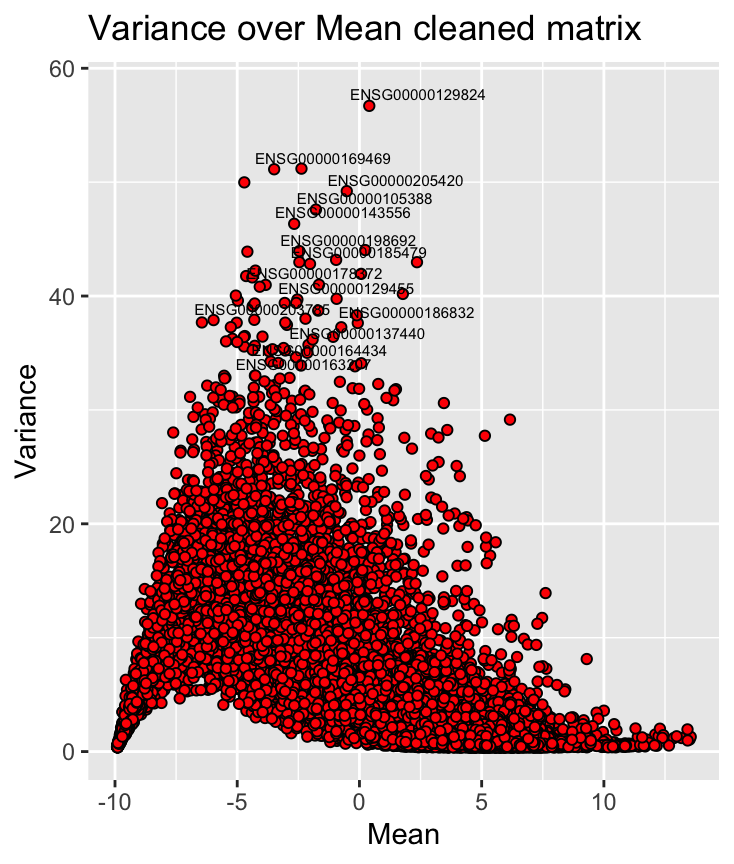
\includegraphics[width=0.3\linewidth]{figures/Variance_over mean_cleaned_matrix} 

}

\caption{Mean-variance plot of cleaned TCGA expression data. Y-axis shows variance of a genes expression, x-axis shows mean of a genes expression}\label{fig:showmeanvariance}
\end{figure}

\hypertarget{significantly-up--and-down-regulated-genes-in-thca-obtained-from-volcano-plots}{%
\subsubsection{Significantly up- and down regulated genes in THCA
obtained from volcano
plots}\label{significantly-up--and-down-regulated-genes-in-thca-obtained-from-volcano-plots}}

To determine those genes that are up- or down-regulated in THCA, the
expression data from tumor tissue was compared to the data from normal
tissue by mean log2 fold change. Associated p-Values were comuted with a
Wilcoxon rank sum test. (Figure @ref(fig:showvolcanoplot)). The
significance level adjusted to 1.755e-06 with a Bonferrioni adjustment.
(!!!!! WICHTIG Welche sind up-regulated, welche down-regulated???)xxx

\begin{figure}

{\centering 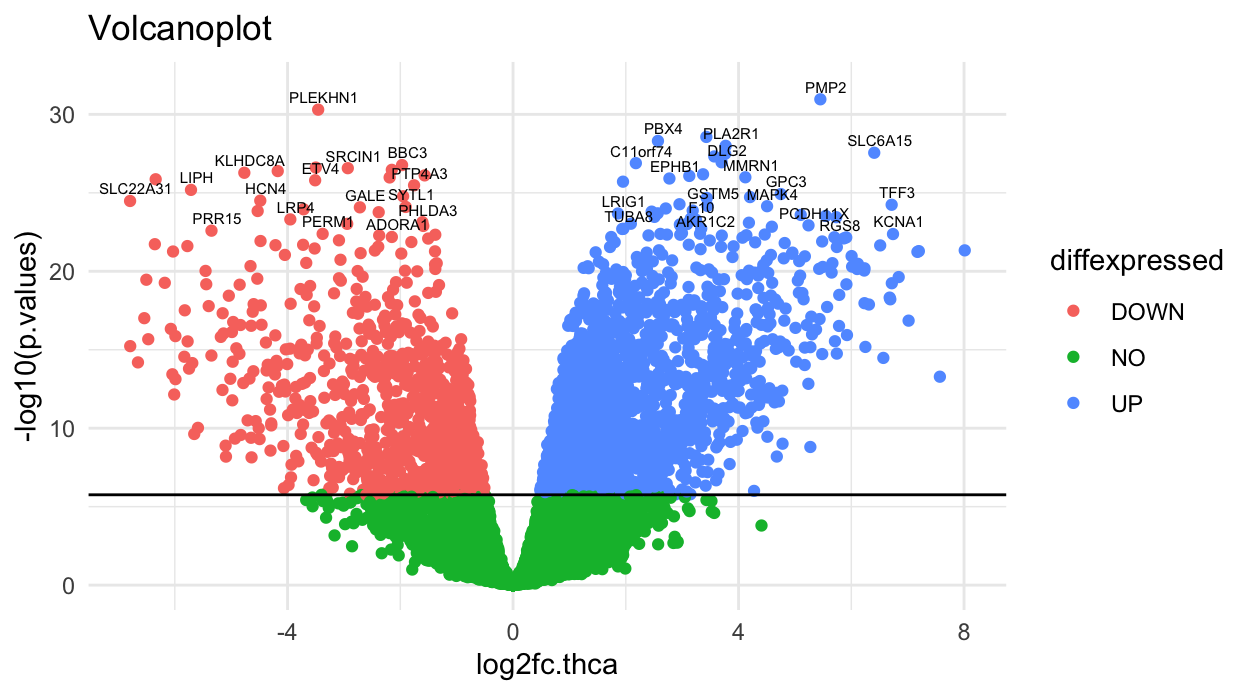
\includegraphics[width=0.3\linewidth]{figures/Volcanoplot} 

}

\caption{Volcano plot of THCA expression data}\label{fig:showvolcanoplot}
\end{figure}

\hypertarget{pan-cancer-analysis}{%
\subsection{Pan cancer analysis}\label{pan-cancer-analysis}}

\hypertarget{gsva-of-tcga-expression-data-reveals-four-clusters-of-cancer-types}{%
\subsubsection{GSVA of TCGA expression data reveals four clusters of
cancer
types}\label{gsva-of-tcga-expression-data-reveals-four-clusters-of-cancer-types}}

To find general clusters a heatmap with the mean expression of each gene
in each tumor type was generated and clustered hierarchically. Figure
@ref(fig:meanexp)

The tumor types were clustered based on their mean pathway activity and
formed four clusters correlating with their histological type. The first
cluster contains mainly adenocarcinamas, while the second one contains
predominately glioblastomas. Leukemias are only found in the third
cluster and the last cluster is enriched with sarcomas and carcinomas.
Melanomas appear in the second and fourth cluster.

Furthermore, three observations were made regarding specific information
about pathway activity.

Pathways, which are important for nucleus import and export like
Nasopharygeal carcinoma (NPC) and Ran shuttle pathways, as well as
pathways for transcription regulaturs in embryonic stem cells are
down-regulated in glioblastoma and adenocarcinoma. However, these
pathways are up-regulated in all other histological types. This
seperation into two clusters is in line with the research of Ben-Porath
et al., that shows an embryonic stem cell-like gene expression only in
poorly differentiated tumors, such as leukemia {[}@result5{]}. In that
way it could be conluded that the differentation stage of a tumor
correlates with pathway activty specific to certain histological types
@ref(fig:meanexp).

Another observation is the clustering of glioblastoma. Pathways
initiating neurogenesis and pathways linked to differentiation of the
neural crest are up-regulated only in glioblastoma {[}@result6{]}. Two
other pathways, that are up-regulated in glioblastoma cells are pathways
linked to the activity of tyrosine kinases. The up-regulation of
tyrosine kinases promote cell growth and proliferation. {[}@cell{]}.
Taken together these two observations are in line with the expected high
proliferation rate commonly found in glioblastoma.

The third cluster is mainly related to adenocarcinomas, more
specifically liver hepatocellular carcinoma (LIHC), kidney renal
papillary cell carcinoma (KICH) and kidney renal clear cell carcinoma
(KIRC). The up-regulated pathways are involved in metabolism of
carbohydrates, synthesis of lipids, synthesis of amino acids and
detoxification. An up-regulation of all of these pathways may lead to
cell growth and proliferation, due to higher metabolic activity,
providing more biomass and energy.

\begin{figure}

{\centering 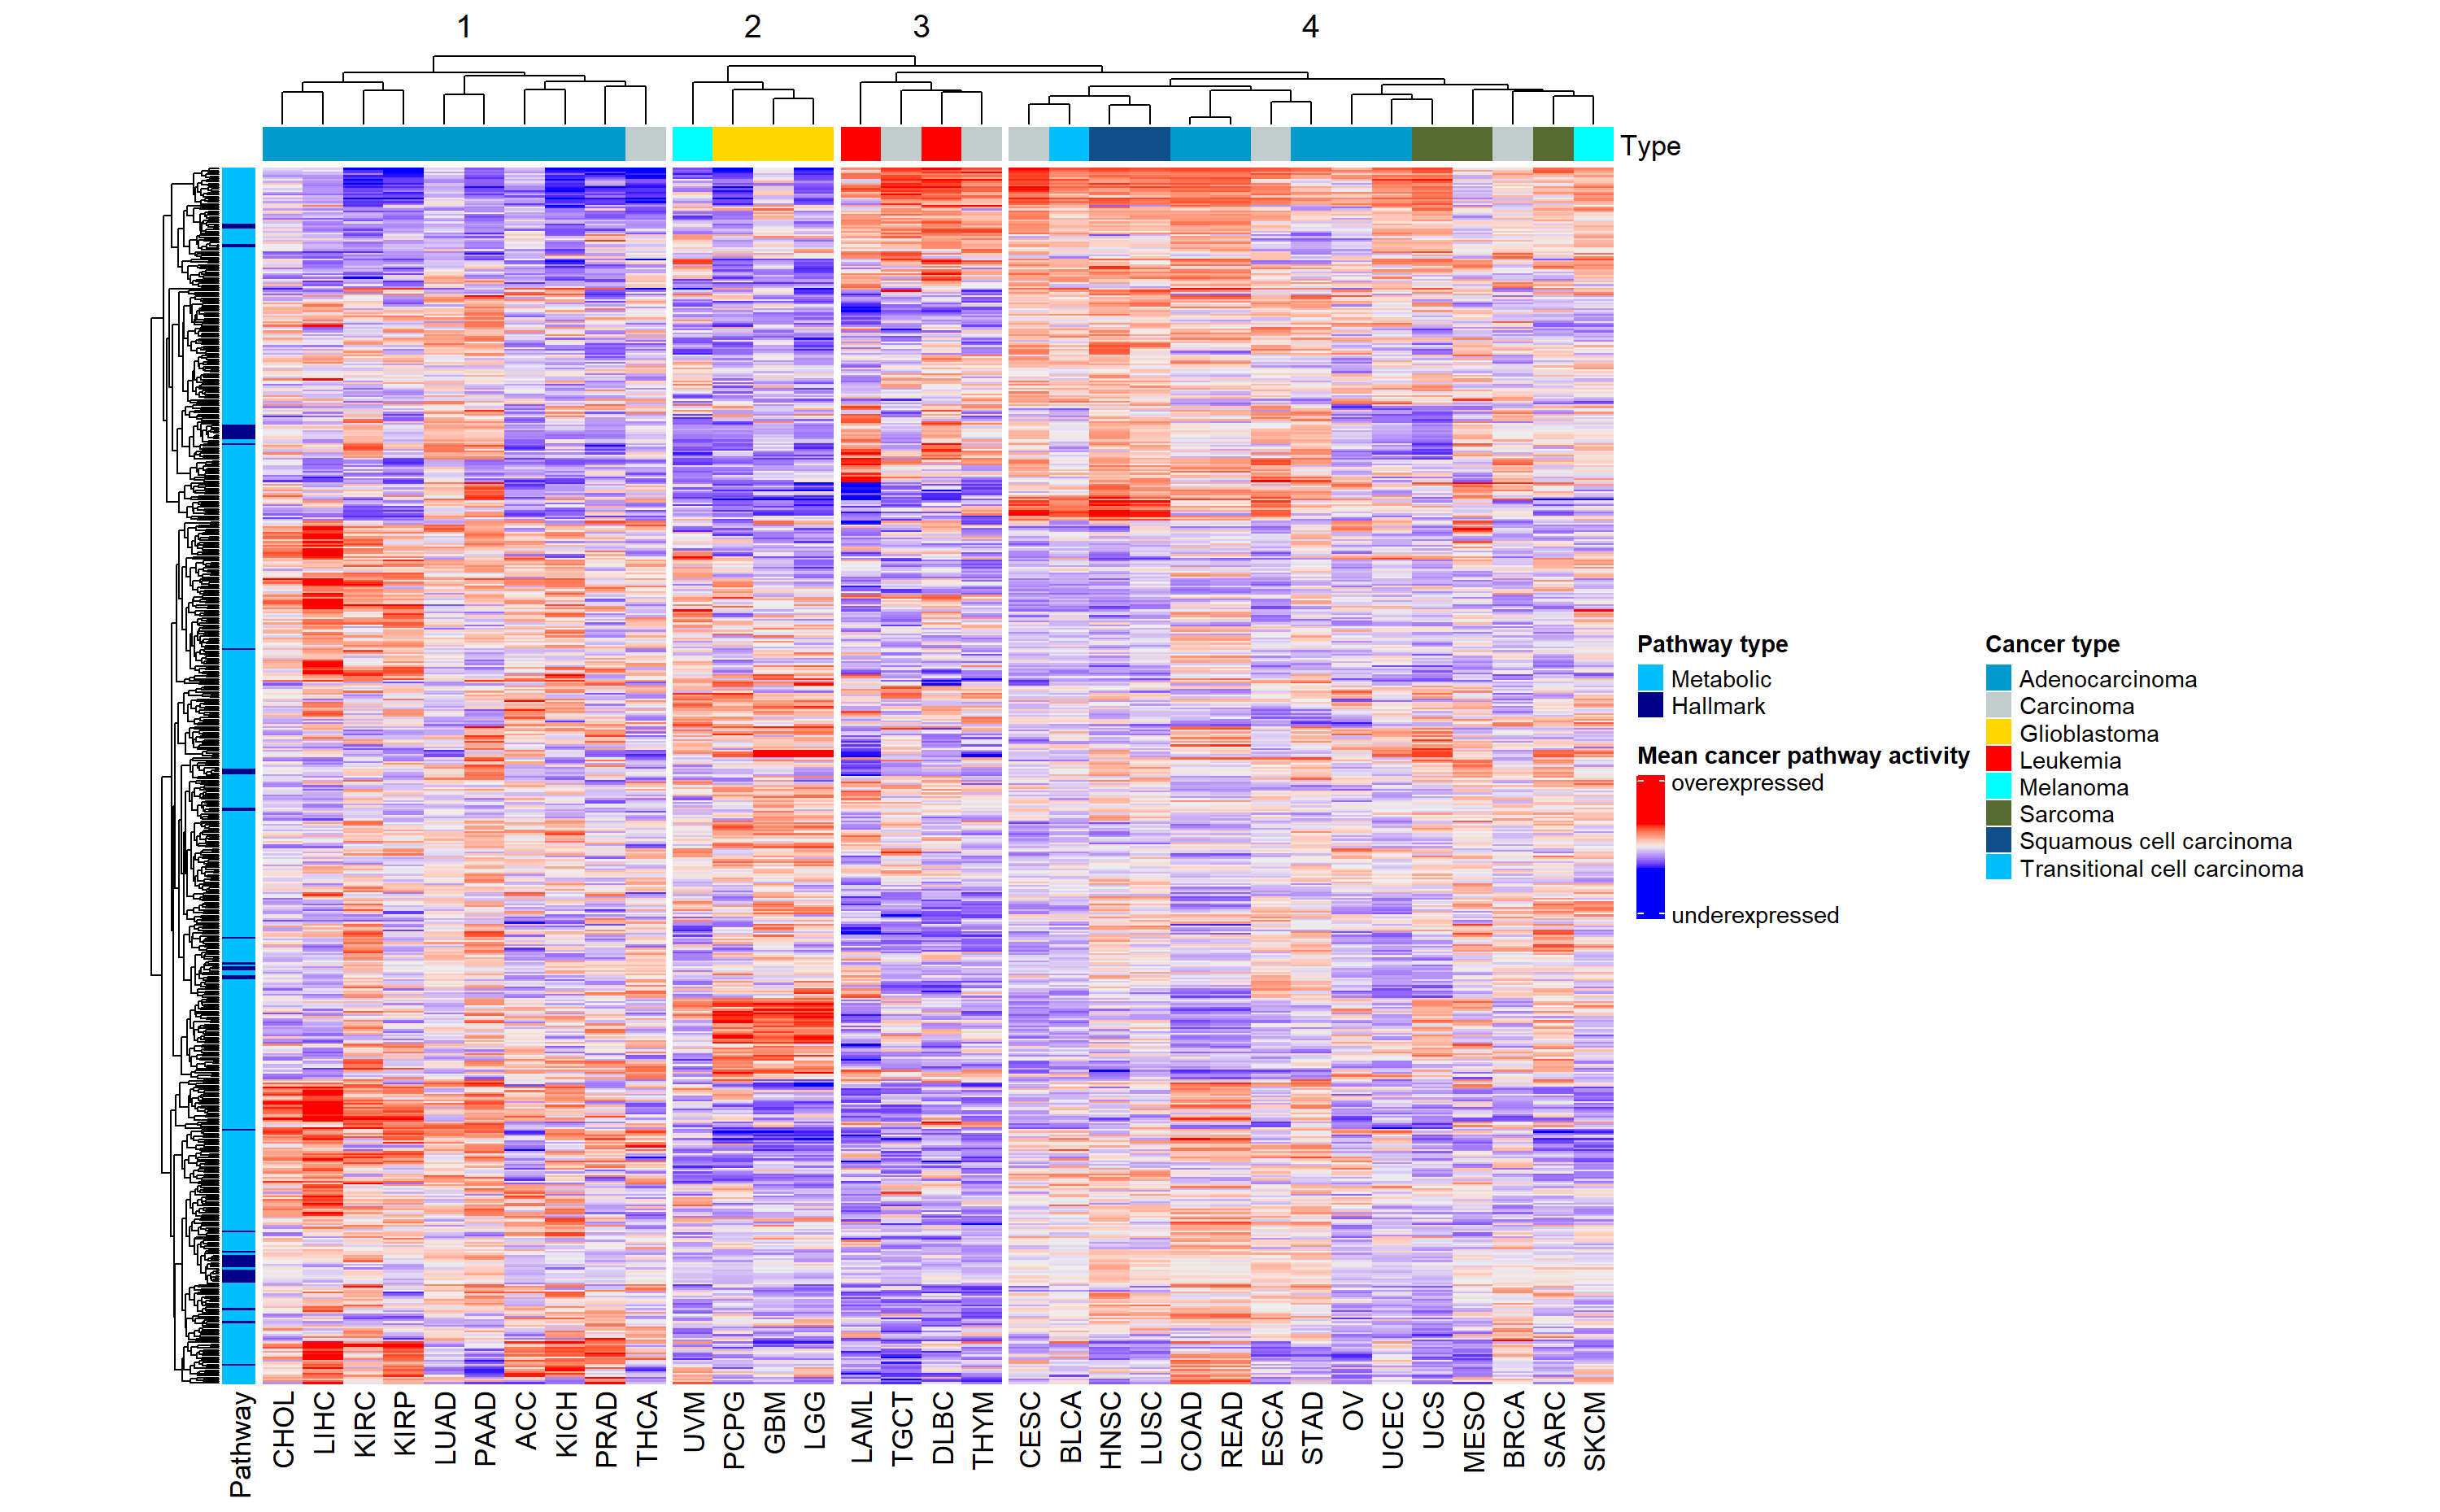
\includegraphics[width=0.5\linewidth]{figures/Pan Cancer mean expression} 

}

\caption{Mean expression of each pathway in each tumot type, annotated with pathway type, histological cancer type and clusters.}\label{fig:meanexp}
\end{figure}

\hypertarget{pca}{%
\subsubsection{PCA}\label{pca}}

\hypertarget{dimension-reduction-of-gsva-pan-cancer-data-reveals-clusters-in-pathway-activity}{%
\subsubsection{Dimension reduction of GSVA pan-cancer data reveals
clusters in pathway
activity}\label{dimension-reduction-of-gsva-pan-cancer-data-reveals-clusters-in-pathway-activity}}

PCA was performed on GSVA pan-cacner data to provide uncorrelted
varibales for better UMAP analysis. No apparent clustering was observed
only in PCA data (compare Figure xxx supplementray materail). Subsequent
UMAP analysis however, showed clear clusters for most cancer types.
@ref(fig:UMAPPanType) @ref(fig:UMAPPanForm). This complemetns the
results obtained from our heatmap and reassures, that the tumor types
have characteristic pathway activities. However, some cancers cluster
better with their histological type rather than tumor type. This was
observed mainly for carcinomas like squamous cell carcinoma and
transitional cell carcinoma, as well as sarcoma, lung adenocarcinoma and
ovarian cancer. These are the same histological types that proofed
difficult to cluster in the mean GSVA of TCGA expression. The UMAP
confirmed the assumption, that the histological type of a tumor has a
major impact on the patients gene expression profile.

\begin{figure}

{\centering 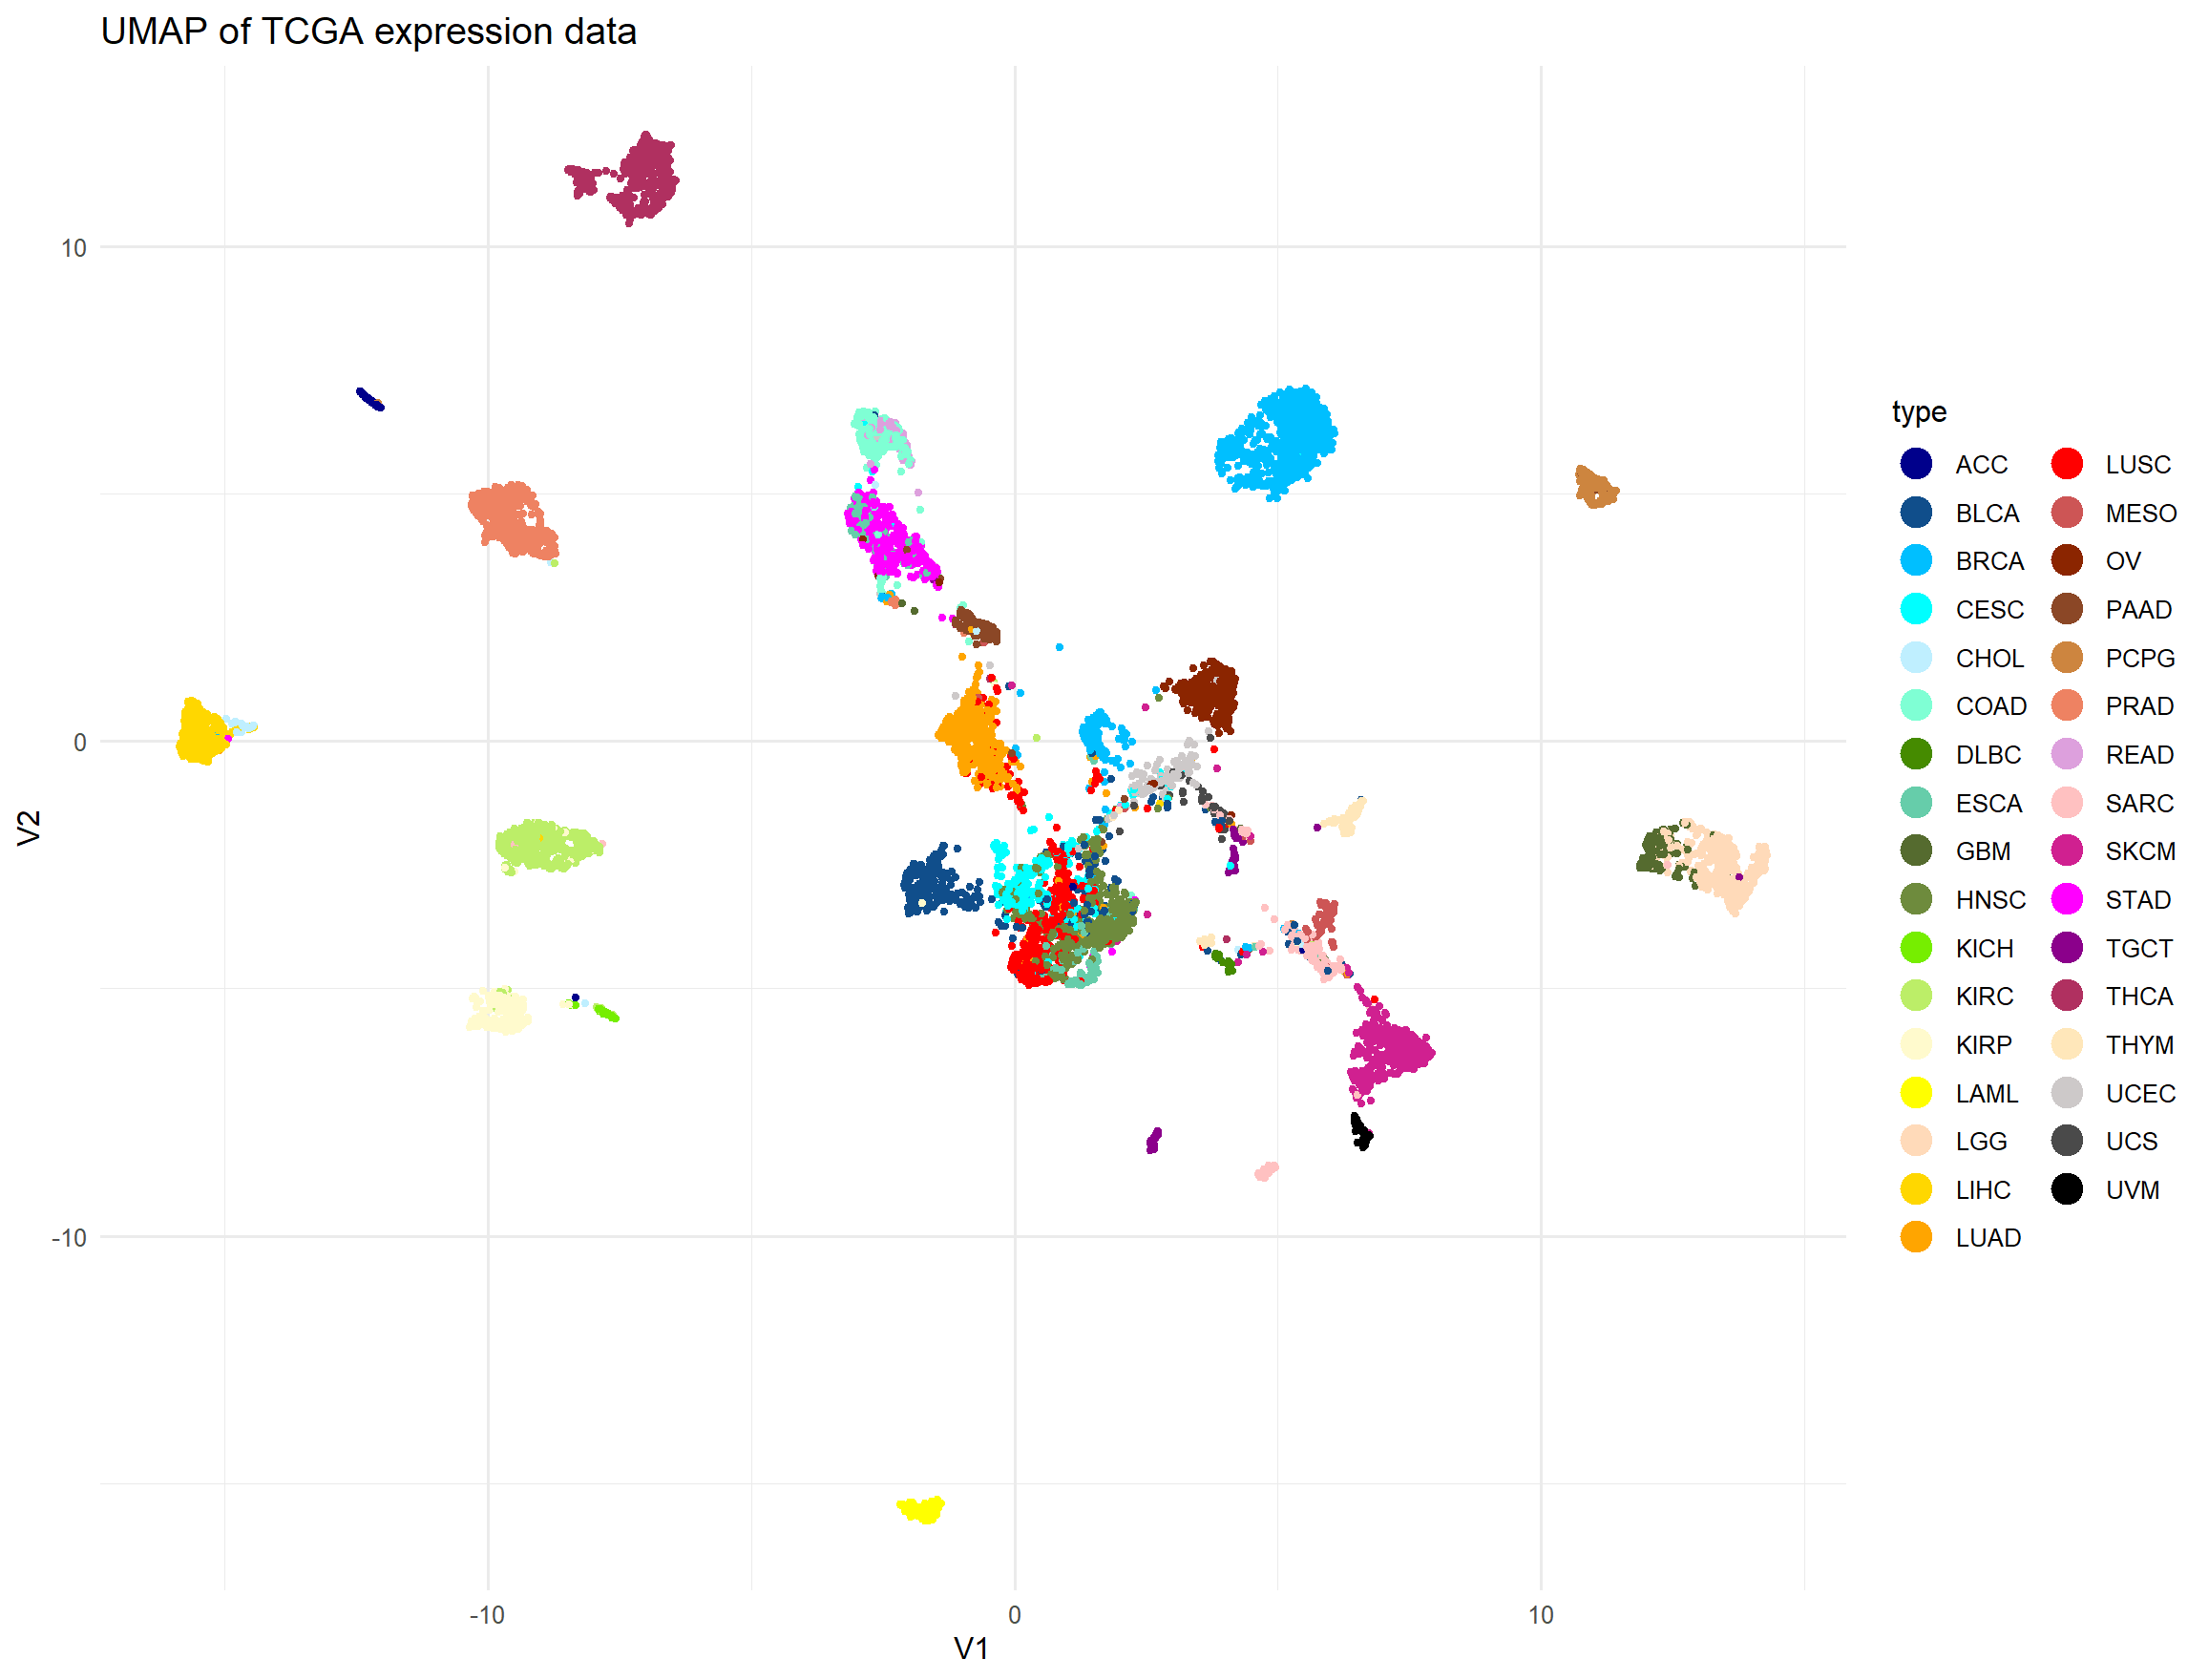
\includegraphics[width=0.5\linewidth]{figures/Pan Cancer UMAP} 

}

\caption{UMAP of TCGA expression data, colored by tumor type}\label{fig:UMAPPanType}
\end{figure}

\begin{figure}

{\centering 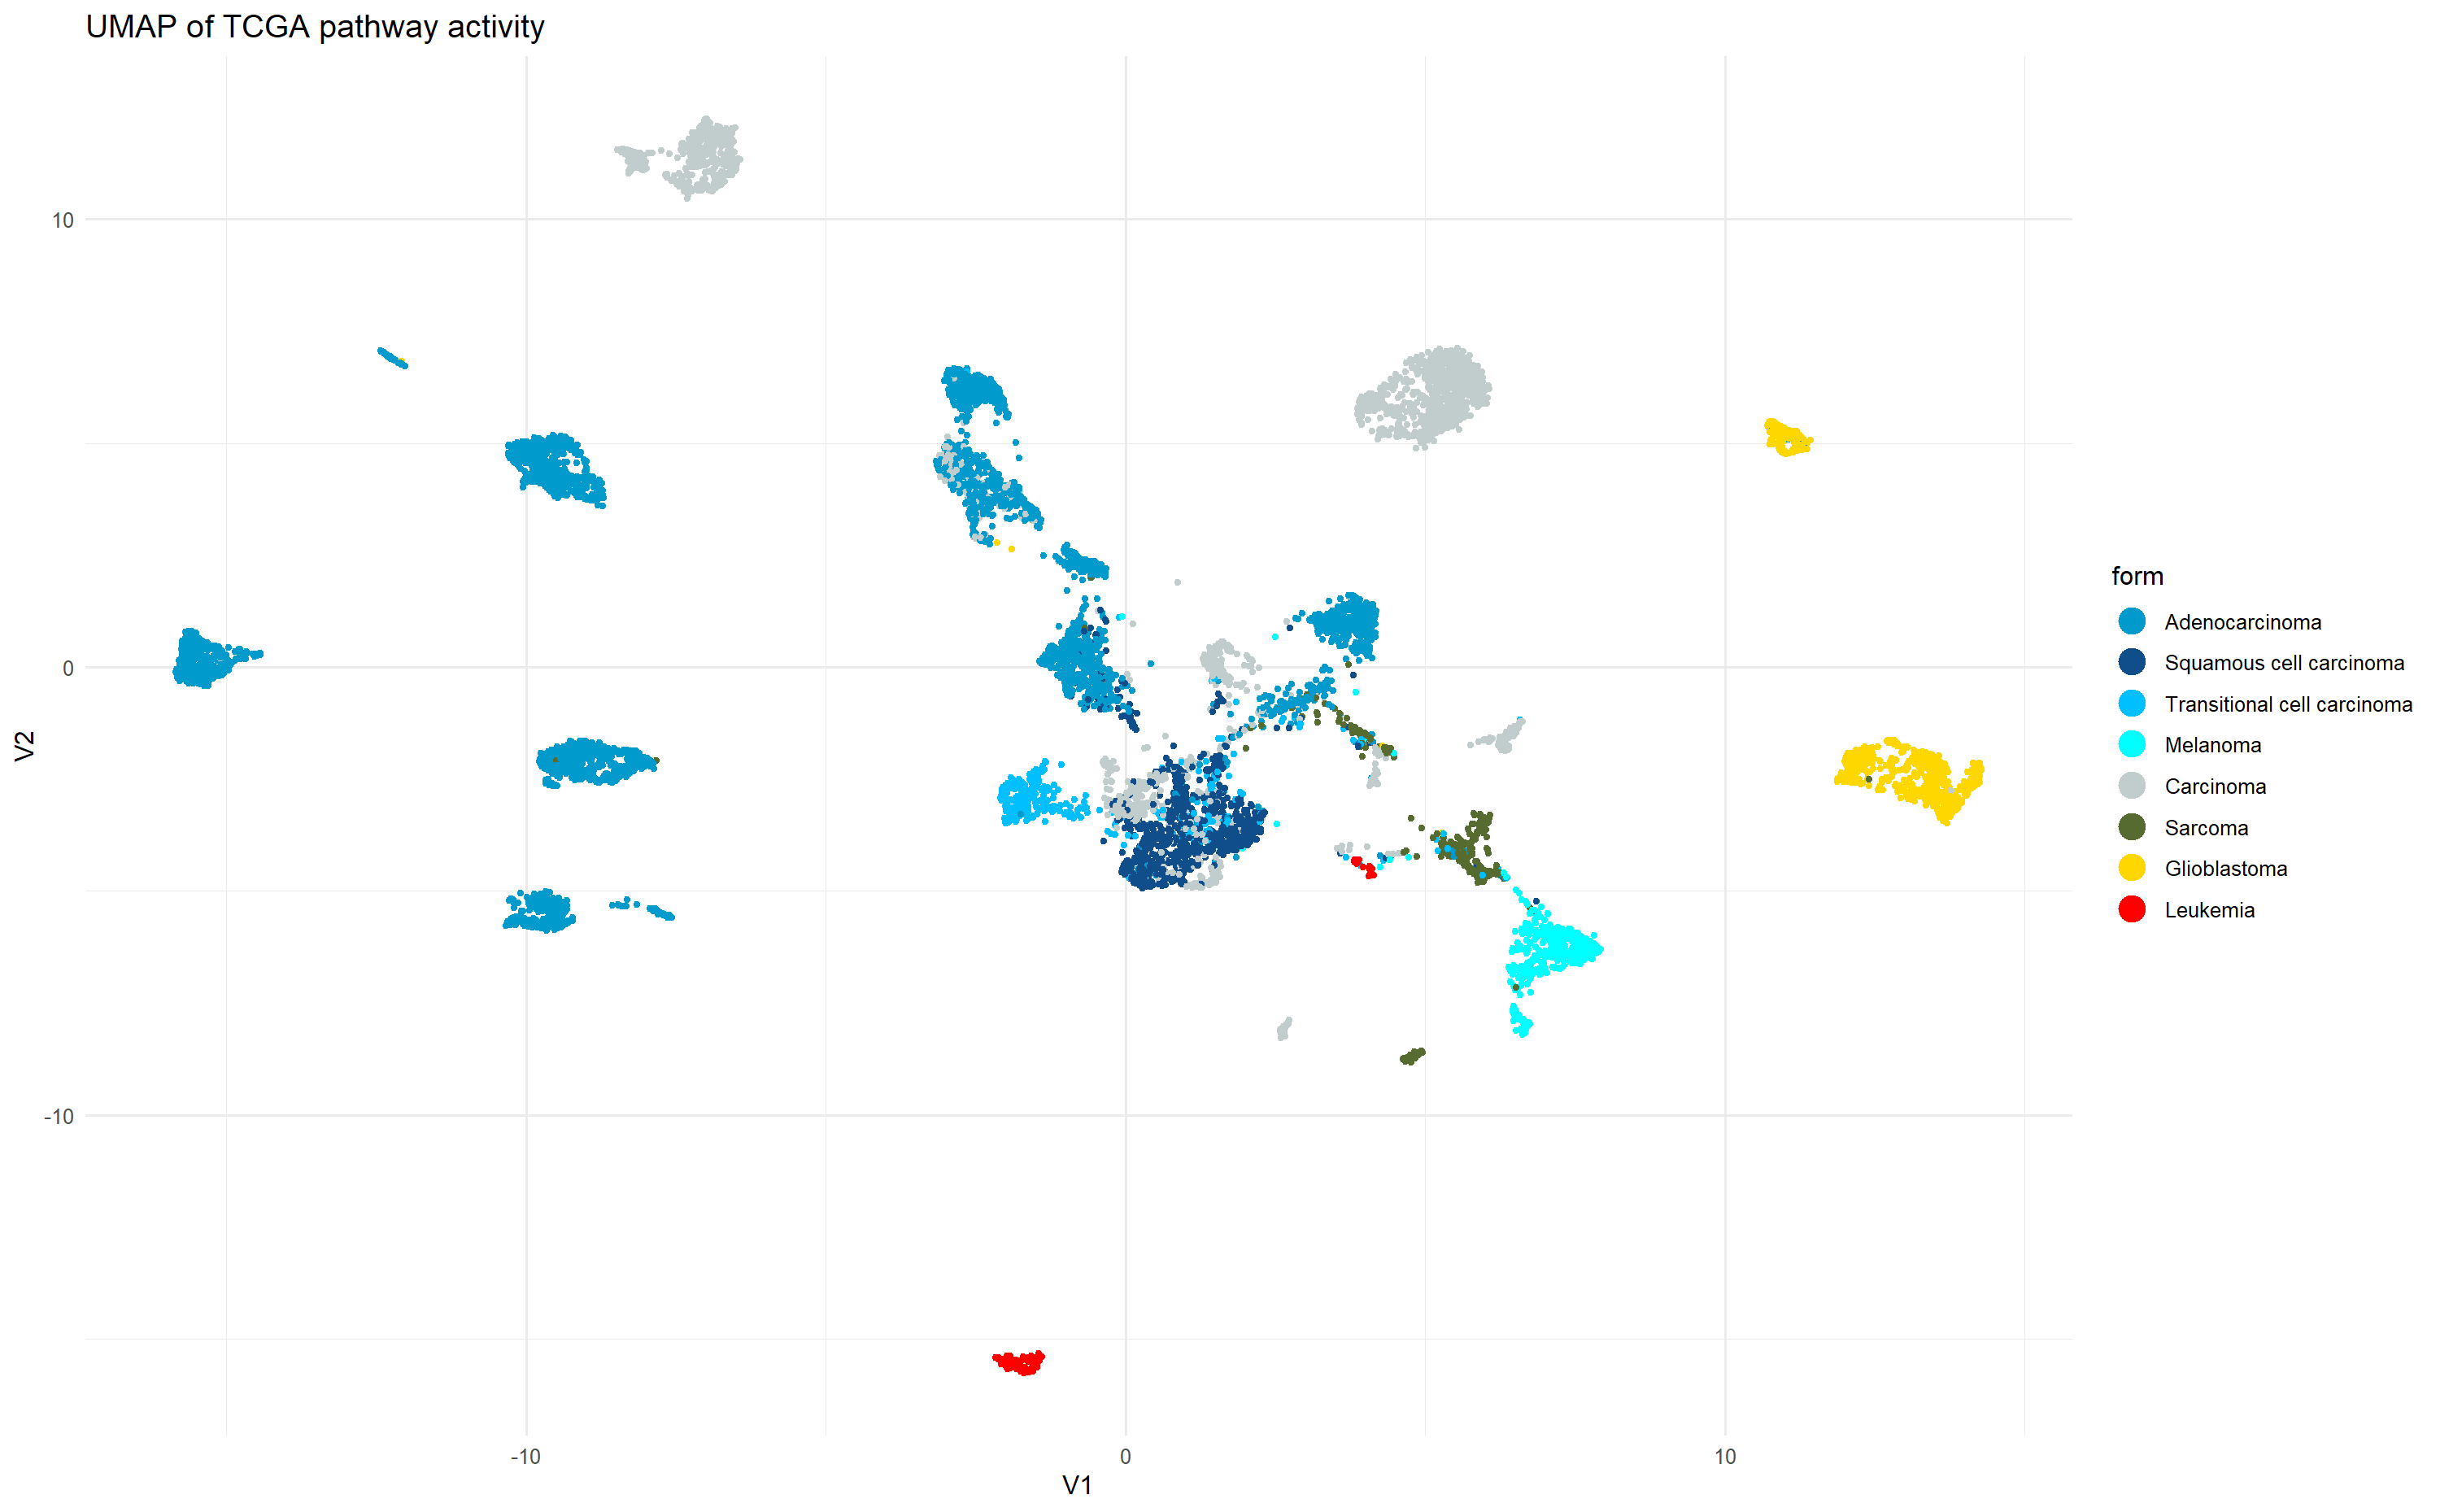
\includegraphics[width=0.5\linewidth]{figures/Pan Cancer UMAP cancer form} 

}

\caption{UMAP of TCGA expression data, colored by form of the tumor}\label{fig:UMAPPanForm}
\end{figure}

The same analysis was performed for gene expression activity instead of
pathway activity to check for reliability of the results. Similar
clusters were observed, which confirms our results (see Fig.
appendix)xxx.

\hypertarget{focused-analysis}{%
\subsection{Focused analysis}\label{focused-analysis}}

\hypertarget{gsva-on-thca-expression-data-reveals-pathways-driving-thyroid-carcinogenesis.}{%
\subsubsection{GSVA on THCA expression data reveals pathways driving
thyroid
carcinogenesis.}\label{gsva-on-thca-expression-data-reveals-pathways-driving-thyroid-carcinogenesis.}}

To grasp a general overview of the differences in pathway activity
between THCA and homeostatic thyroid tissue, GSVA was performed for the
THCA expression data. Then, changes in pathway activity were computed by
log2 fold change and the respective p-values were computed by a Wilcoxon
rank-sum test. The most significantly altered pathways were then
characterized. Most prominently among them were pathways linked to
proliferative signaling such as upregulation of p53 inhibitory proteins
and hedgehog pathway activating Gli proteins. Further, the alpha6beta4
integrin signaling pathway and associated pathways such as IL-36
signaling and Typ I hemidesmosome synthesis were significantly enhanced
in THCA. These findings are consistent with previous studies that linked
alpha6beta4 signaling to the development of aggressive forms of thyroid
cancer {[}@result4,@result3{]}. Also, oncogenic signaling pathways
commonly associated with different cancer types were significantly
upregulated in THCAs. Among them, we observed ERBB2 QUELLE MSigDB and
MST1 signaling commonly found in breast cancer. A role for MSP/Ron in
breast cancer has recently been elucidated, wherein this pathway
regulates tumor growth, angiogenesis, and metastasis {[}@result2{]}.

Further, signaling through the EWSR1/FL1-fusion protein was
significantly upregulated in THCA and previously shown to promote the
rapid development of myeloid/erythroid leukemia in mice Quelle Msigdb.
Lastly, THCAs showed downregulation of non-histone protein methylation.
This process was identified as an import modulator of intracellular
signaling by the MAPK, WNT, BMP, Hippo, and JAK/STAT pathways and might
play an important role as a driver of carcinogenesis in THCA
{[}@result1{]}. Together these findings give a general overview of
mechanisms driving carcinogenesis in THCA. However, no information about
possible THCA subtypes or differences in patway activity between
patients can be obtained from this data.

\hypertarget{pan-cancer-data-gsva-reveals-three-subtypes-of-thca-altering-in-proliferative-signaling.}{%
\subsubsection{Pan-cancer data GSVA reveals three subtypes of THCA
altering in proliferative
signaling.}\label{pan-cancer-data-gsva-reveals-three-subtypes-of-thca-altering-in-proliferative-signaling.}}

To investigate potential subtypes of THCA, the respective samples were
taken from the pan-cancer GSVA data. The optimal number of clusters was
determined by an elbow plot and subsequent K-means clustering revealed a
total of three subtypes in THCA. This is consistent with the three
clusters of THCA observed in the full pan-cancer GSVA data. The
follicular histological type was enriched in cluster B, with no tall
cell types present in this cluster. Judging from histological type alone
no difference in clusters A and C was observed. Most significant changes
in pathway activity were observed in pathways concerning proliferative
signaling. In comparison with all other tumor types, cluster A displayed
high activity of RAS, JAK/STAT and EWSR1/FL1-fusion mediated signaling
as well as elevated signatures associated with carcinogenesis driven by
alpha6beta4 activity. In contrast, these pathways were downregulated in
cluster B, with it showing elevated activity in mTOR, MAPK, PI3K, and
EGFR signaling cascades. Cluster C was found to upregulate all the
aforementioned forms of proliferative signaling. All clusters showed a
homogenous upregulation of hedgehog, ERBB2, and MST1 pathway activity.
Regarding immune response, cluster C showed no significant alterations
in the respective hallmark pathways, however, these pathways were
downregulated in both clusters A and B. With this data, we can identify
two seemingly different forms of proliferative signaling driving
carcinogenesis in THCA. These forms can either occur separately as in
the case of clusters A and B or combined as for cluster C.

\hypertarget{thca-subtypes-do-not-differ-in-their-metabolism.}{%
\subsubsection{THCA subtypes do not differ in their
metabolism.}\label{thca-subtypes-do-not-differ-in-their-metabolism.}}

To investigate how the identified subtypes compare to homeostatic
thyroid tissue, GSEA was performed for the THCA data. Consistent with
the pan-cancer analysis of THCA data, k-means clustering obtained three
different clusters in pathway activity -- verified as the optimal number
of clusters via an elbow plot. All clusters showed a similar change in
metabolism. Katabolic pathways are downregulated whereas anabolic
pathways e.g., fatty acid synthesis show increased activity in
comparison with normal tissue. These changes in metabolic activity are
in line with the Warburg effect. Further, the results seem consistent
with the proliferative signaling activities found previously.
Alpha6beta4, RAS, JAK/STAT, and EWSR1/FL1-fusion mediated signaling is
upregulated in clusters one and three with low expression in cluster
two. However, the expected upregulation of mTOR, MAPK, PI3K, and EGFR
signaling in clusters two and three was observed only in some samples.
Regarding, immune response the expression profiles are again consistent
with differences observed in the GSVA pan-cancer data: Both clusters one
and two show a lower immune response compared to cluster three. From
these GSEA results, we can conclude that the three subtypes of THCA
differ in carcinogenesis and associated immune response but share a
similar metabolism consistent with the Warburg effect.

\hypertarget{regression-analysis-of-thca-pathway-activity}{%
\subsection{Regression analysis of THCA pathway
activity}\label{regression-analysis-of-thca-pathway-activity}}

To select a suitable pathway for regression analysis, the top 20\%
pathways regarding their variance in activity were chosen, as for the
regression model to predict. Pathways with little variance were found to
be better predicted by a null model (Fig xxx supplementary material). To
factor in biological significance, the intersect of the 25 most
significantly altered pathways from GSVA with the high variance pathways
was computed. This resulted in three significantly altered and highly
variant pathways among which the REACTOME\_INTERLEUKIN\_36\_PATHWAY gene
set was selected. This gene set ranks 8th among the highest upregulated
pathways with an associated p-value of 8.411155e-15. As interleukin 36
signaling is connected to both MAPK activity and through the activation
of NF-kB also the expression of integrin alpha6beta4 effective
regression might be crucial in finding potentially druggable targets in
combating THCA{[}@result4{]} Msigdb xxx. Parathyroid hormone-related
protein regulates integrin α6 and β4 levels via transcriptional and
post-translational pathways Regression of the
REACTOME\_INTERLEUKIN\_36\_PATHWAY gene set showed mixed results.

As expected, the neuronal network performed best on the test data with a
mean squared error (MSE) of 0.06. However, the linear regression model
failed to predict the data accurately (MSE = 0.62). Repeated linear
regression with just pathways contributing significantly to the result
the performance was enhanced (MSE = 0.40), however, remained worse than
a null model (MSE = 0.22). (Fig. xxx) A comparison of the four
regression models via the F-test function \texttt{\{var.test()\}} showed
a significant improvement of the neuronal network compared to all other
models. All other models showed no significant differences in their
performance (Fig. xxx) compared to each other. From this data, we can
conclude that a neuronal network is the best choice for most accurately
predicting IL-36 pathway activity in our test data.

\end{document}
